%% LyX 2.3.7 created this file.  For more info, see http://www.lyx.org/.
%% Do not edit unless you really know what you are doing.
\documentclass[a4paper,oneside,french]{amsart}
\usepackage[T1]{fontenc}
\usepackage[utf8]{inputenc}
\setlength{\parskip}{\smallskipamount}
\setlength{\parindent}{0pt}
\synctex=1
\usepackage{babel}
\makeatletter
\addto\extrasfrench{%
   \providecommand{\og}{\leavevmode\flqq~}%
   \providecommand{\fg}{\ifdim\lastskip>\z@\unskip\fi~\frqq}%
}

\makeatother
\usepackage{float}
\usepackage{amstext}
\usepackage{amsthm}
\usepackage{amssymb}
\usepackage{wasysym}
\usepackage[unicode=true,pdfusetitle,
 bookmarks=true,bookmarksnumbered=false,bookmarksopen=false,
 breaklinks=false,pdfborder={0 0 1},backref=false,colorlinks=false]
 {hyperref}

\makeatletter

%%%%%%%%%%%%%%%%%%%%%%%%%%%%%% LyX specific LaTeX commands.
\pdfpageheight\paperheight
\pdfpagewidth\paperwidth


%%%%%%%%%%%%%%%%%%%%%%%%%%%%%% Textclass specific LaTeX commands.
\numberwithin{equation}{section}
\numberwithin{figure}{section}

%%%%%%%%%%%%%%%%%%%%%%%%%%%%%% User specified LaTeX commands.
\usepackage{tikz}

\makeatother

\usepackage{listings}
\renewcommand{\lstlistingname}{\inputencoding{latin9}Listing}

\begin{document}
\title{Projet de stage: traduction automatique de documents LateX}
\author{Matthieu Boileau, Philippe Helluy}
\address{IRMA Université de Strasbourg, Inria Tonus}
\email{philippe.helluy@unistra.fr}
\begin{abstract}
Il s'agit de la description d'un projet de stage de L2, visant à développer
un logiciel pour la traduction automatique de documents scientifiques
écrits dans le langage LaTeX. 
\end{abstract}

\keywords{LaTeX, traduction automatique, mathématiques}
\maketitle

\section{Objectifs}

LaTeX est un système d'écriture de documents qui est très utilisé
dans le milieu scientifique. L'objectif du stage est de réaliser un
logiciel python de traduction automatique d'un fichier LaTeX d'une
langue vers une autre. La difficulté est que le document va contenir
des formules mathématiques ou d'autres structures dans certains paragraphes.
Il faut maintenir ces structures dans la traduction pour que celle-ci
soit de bonne qualité.

On trouve déjà (mai 2023) plusieurs tentatives de réalisation de ce
type de logiciel sur le web. On peut citer par exemple \cite{ohri2021machine,gtexfix}.

Voici les fonctionnalités attendue du logiciel:
\begin{itemize}
\item Logiciel en ligne de commandes. Exemple: \inputencoding{latin9}
\begin{lstlisting}[language=bash]
translatex article_fr.tex article_en.tex
\end{lstlisting}
\inputencoding{utf8} ou \inputencoding{latin9}
\begin{lstlisting}[language=bash]
translatex article_fr.lyx article_en.lyx
\end{lstlisting}
\inputencoding{utf8}La langue est indiquée dans le nom du fichier.
\item Traduction des textes inclus dans les structures \texttt{\textbackslash text\{...\}}
des formules.
\item Laisser \emph{inchangées} les structures non reconnues (en les indiquant
en rouge, par exemple). Le programme ne doit pas \textbf{bloquer}
sur des erreurs.
\item Possibilité d'utiliser plusieurs services en ligne, comme Google,
DeepL, \href{https://textsynth.com/}{https://textsynth.com/}, \href{https://dlmds.math.unistra.fr/}{https://dlmds.math.unistra.fr/}.
\end{itemize}

\section{Plan de travail}

Le plan de travail ci-dessous est indicatif, il peut évoluer en fonction
des avancées du projet.
\begin{enumerate}
\item Faire de la bibliographie et de la recherche sur le web. Inutile de
refaire ce qui existe déjà en mieux. Rédiger un petit état de l'art.
\item Faut-il utiliser les expressions régulières ou un analyseur de syntaxe
plus sophistiqué comme \cite{pylatexenc} ? 
\item En prenant comme exemple le texte de ce document, faire la liste des
structures qui doivent être traduites correctement. Par exemple: titre,
résumé, italique, gras, 
\item Réfléchir à une structure modulaire du code. Il doit être facile de
pouvoir ajouter la gestion de nouveaux patterns.
\end{enumerate}

\section{Annexe: exemple de texte à traduire}

Cette section contient plusieurs types de structures (formules, tableaux,
images), afin de fournir un exemple de texte à traduire.

Soit la matrice 
\begin{equation}
A=\left[\begin{array}{ccc}
3 & 3 & 4\\
6 & -2 & -12\\
-2 & 3 & 9
\end{array}\right].\label{eq:A}
\end{equation}

\begin{enumerate}
\item Diagonaliser cette matrice: trouver une matrice de passage $P$ et
une matrice diagonale
\[
D=\left[\begin{array}{ccc}
\lambda_{1} & 0 & 0\\
0 & \lambda_{2} & 0\\
0 & 0 & \lambda_{3}
\end{array}\right],
\]
avec $\lambda_{1}<\lambda_{2}<\lambda_{3}$ tels que
\[
D=P^{-1}AP.
\]
On note $e_{j}$ la $j$-ème colonne de $P$. Que peut-on dire de
$e_{j}$ ?
\item Écrire un programme Python utilisant numpy qui permet de retrouver
la plus grande et la plus petite valeur propre d'une matrice $A$
au moyen de la méthode de la puissance itérée, ainsi que des vecteurs
propres associés.
\item Soit $\gamma:[0,1]\to\mathbb{C}$ une application régulière, telle
que $\gamma(0)=\gamma(1)$. On note $\Gamma$ la courbe paramétrée
engendrée par $\gamma$, $\Gamma=\gamma([0,1]).$ Écrire un programme
Python qui représente la courbe obtenue avec matplotlib lorsque
\begin{equation}
\gamma(t)=\exp(2i\pi t),\quad i^{2}=-1.\label{eq:contour}
\end{equation}
\item \label{enu:q4}On considère maintenant une application $f$ de $\mathbb{C}$
dans $\mathbb{C}$. On définit l'intégrale de $f$ sur le contour
$\Gamma$ par la formule
\begin{equation}
\varoint_{\Gamma}f(z)dz=\int_{t=0}^{1}f(\gamma(t))\gamma'(t)dt.\label{eq:int_contour}
\end{equation}
Calculer cette intégrale de contour lorsque $f(z)=(z-z_{0})^{3}$,
$z_{0}=\frac{1+i}{2}$ et que $\gamma$ est donné par (\ref{eq:contour}).
Même question pour $f(z)=1/(z-z_{0})$.
\item \label{enu:intnum}Écrire un programme Python qui calcule l'intégrale
(\ref{eq:int_contour}) par la méthode des rectangles à gauche. Vérifier
que dans ce cas (sur les deux exemples de la question \ref{enu:q4}),
la méthode est d'ordre $>1$. Pourquoi ? (Indications: \cite{helluy1998integration})
\item \label{enu:q6}On définit le projecteur $\Pi_{j}$ sur l'espace propre
associé à $\lambda_{j}$ de la façon suivante. On considère la matrice
diagonale $J_{j}$ définit par
\[
\left(J_{j}\right)_{k,l}=\begin{cases}
1 & \text{si }j=k=l,\\
0 & \text{sinon}.
\end{cases}
\]
Puis
\[
\Pi_{i}=PJ_{i}P^{-1}.
\]
Soit une matrice $A$ de taille $n\times n$ dont les valeurs propres
sont notées $\lambda_{j}$, $i=1\ldots n$. Soit un contour $\Gamma$.
On suppose que $\Gamma$ est la frontière d'un ouvert $\Omega$ du
plan complexe: $\Gamma=\partial\Omega$, que $\gamma$ fait le tour
de $\Omega$ dans le sens trigonométrique et que $\gamma$ n'a pas
d'autre point double que $0$ et $1$: 
\[
\forall s,t\in]0,1],s\neq t\Rightarrow\gamma(s)\neq\gamma(t).
\]
On note $K$ l'ensemble des indices des valeurs propres qui sont entourées
par le contour $\Gamma$:
\[
K=\left\{ k,\lambda_{k}\in\Omega\right\} .
\]
Voir exemple sur la Figure \ref{fig:contour}.
\begin{figure}[H]
\begin{centering}
\begin{center}
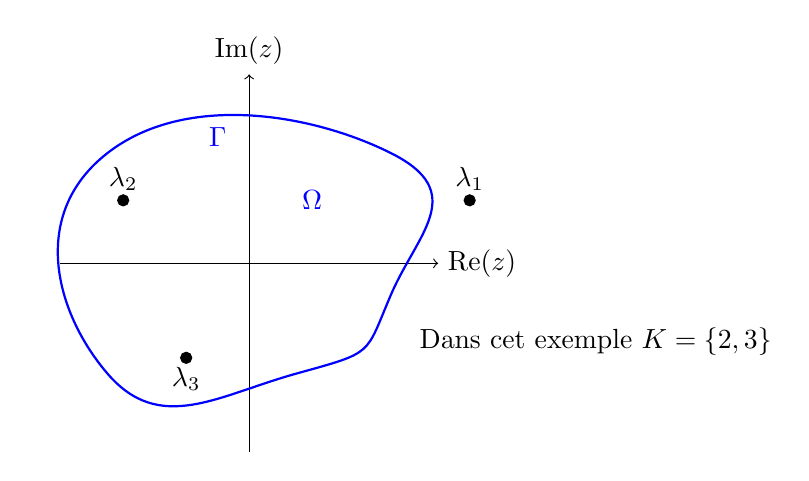
\begin{tikzpicture}[scale=2]

% Axes
\draw[->] (-1.2,0) -- (1.2,0) node[right] {$\mathrm{Re}(z)$};
\draw[->] (0,-1.2) -- (0,1.2) node[above] {$\mathrm{Im}(z)$};

% Points
\draw[black,fill=black] (1.4,0.4) node[above] {$\lambda_1$} circle (1pt);
\draw[black,fill=black] (-0.8,0.4) node[above] {$\lambda_2$} circle (1pt);
\draw[black,fill=black] (-0.4,-0.6) node[below] {$\lambda_3$} circle (1pt);

% Contour
\draw[blue, thick, ->] plot[smooth cycle, tension=1] coordinates {(0.9,0.7) (-0.9,0.7) (-0.9,-0.7) (0.3,-0.7) (0.9,-0.2)};

% Domaine
\node[blue] at (0.4,0.4) {$\Omega$};

% Contour label
\node[blue] at (-0.2,0.8) {$\Gamma$};

\node[black] at (2.2,-0.5)  {Dans cet exemple $K=\left\{2,3\right\}$};

\end{tikzpicture}
\end{center}
\par\end{centering}
\caption{Exemple de contour dans le plan complexe entourant des valeurs propres.\label{fig:contour}}
\end{figure}
On admet le (joli) résultat suivant\footnote{Si $B(t)=(b_{i,j}(t))$ est une matrice dont les éléments dépendent
de $t$, $\int B(t)dt$ est tout simplement la matrice dont les éléments
sont les $\int b_{i,j}(t)dt$.}:
\begin{equation}
\frac{1}{2i\pi}\varoint_{\Gamma}(zI-A)^{-1}dz=\sum_{k\in K}\Pi_{k}.\label{eq:proj_spectrale}
\end{equation}
Vérifier cette formule (avec SymPy) pour la matrice (\ref{eq:A})
et le contour
\[
\gamma(t)=2\exp(2i\pi t)
\]
qui entoure la valeur propre $\lambda_{1}$ (mais pas $\lambda_{2}$
ni $\lambda_{3}$). Voici un exemple de calcul d'intégrale avec SymPy:\\
\inputencoding{latin9}\begin{lstlisting}[language=Python]
import sympy as sp

x = sp.Symbol('x')
f = x**2
int_f = sp.integrate(f, x)

print(int_f)
\end{lstlisting}
\inputencoding{utf8}\item Adapter le programme de la question \ref{enu:intnum} pour calculer
numériquement la formule (\ref{eq:proj_spectrale}). 
\end{enumerate}
\bibliographystyle{plain}
\bibliography{translatex}

\end{document}